\chapter{21/09/16 - Introduzione, parte seconda}
\section{Breve descrizione della lezione}
Parleremo di curve algebriche, ossia luoghi di zeri di polinomi omogenei nel proiettivo complesso. In particolare, menzioneremo la classificazione delle cubiche in forma di weierstrass. Daremo una struttura di gruppo alle cubiche complesse e illustreremo la relazione tra cubiche e tori complessi. Infine, troveremo uno 'spazio dei parametri' per i tori complessi.
\section{Curve algebriche non singolari}

Introduciamo anzitutto il concetto di singolarità.

\notamargine{Il contesto in cui ci troviamo è $\bbP_n(\bbK)$, dove $\bbK$ è un campo che spesso sarà $\bbC$ e $n$ spesso sarà 2.}
Data una curva $\gamma$ descritta come zeri in $\bbP_n(\bbK)$ di $f \in \bbK[x_0, \ldots,x_n]$ omogenea, diciamo che un punto è 
\textit{singolare} se, in un senso che renderemo più preciso, non esiste una sola retta tangente alla curva passante per il punto. \textit{Geometricamente}, un punto $p \in \gamma$ è singolare se esiste più di una retta $r$ passante per $p$ con ordine di contatto $\geq 2$. \notamargine{L'ordine di contatto di $r$ con $\gamma$ in $p$ è la molteplicità di $p$ come zero del sistema $r=0,f=0$.}
\vspace{1em}

%%mettere un disegno con cuspide e nodo
%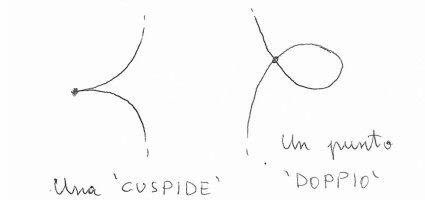
\includegraphics[width=20em]{punti-singolari.jpeg}
\curvegraph{y**2 - x**3 - x**2}{[-2:2]}{[-2:2]}

\textit{Algebricamente}, un punto $p$ zero di $f$ è singolare se $\de{x_i}f(p)=0$ per $i=0,\ldots,n$ (ha il differenziale nullo). \notamargine{Se il campo ha caratteristica 0, notare che $\de{x_i}f(p) = 0$ per ogni $i$ implica $f(p)=0$ per il \href{https://it.wikipedia.org/wiki/Funzione_omogenea}{teorema di eulero} sulle funzioni omogenee.}


\section{Cubiche, forma di Weierstrass}
Nel caso speciale di $n=2$, $\chr \bbK = 0$ c'è un importante risultato di classificazione delle curve non singolari. 
\notamargine{Una curva si dice non singolare se ogni suo punto è non singolare.} 

Consideriamo curve descritte da
$$ zy^2= ax^3+bx^2z+cxz^2+dz^3 $$
 dove $ax^3+bx^2+cx+d$ è un polinomio senza radici multiple, detta \smallcaps{forma di weierstrass}. Allora è non singolare. Imponiamo infatti le tre equazioni:

%% ESERCIZIO: dimostrare che la forma di weierstrass è non singolare

$$ \left\{ 
\begin{matrix}
&3ax^2&+2bxz&+cz^2 & = & -\de{x}f & = 0 \\
&&yz& & = & \de{y}f / 2 &= 0 \\
y^2 &-bx^2&-2cx&-3dz^2 & = & \de{z}f& = 0 \\
ax^3&+bx^2z&+cxz^2&+dz^3& = & zy^2&
\end{matrix}
\right.$$

Dalla (2) abbiamo due casi:

\begin{itemize}
	\item Se $z=0$ allora (4) dà $x=0$ e dunque $y=0$ dalla (3), assurdo.
	\notamargine{ Siamo nel proiettivo: $x=y=z=0$ non è un punto!} 

	\item Se $y = 0$, $z \neq 0$ allora (4) dà $q(x/z) = 0$ e (1) dà $q'(x/z) = 0$ (dove $q$ è il polinomio di coefficienti $a,b,c,d$). Ma allora $x/z$ sarebbe una radice multipla di $q$, assurdo.  
	\notamargine{Infatti se $\chr \bbK = 0$ vale il criterio della derivata.}
\end{itemize}

Viceversa, data una curva cubica non singolare, può essere descritta da un polinomio in forma di weierstrass. Algebricamente, per ogni polinomio omogeneo $f$ di grado 3 con differenziale mai nullo, esiste una $L \in \bbP GL_2(\bbK) $ tale che $f \circ L$ (che è ancora un polinomio omogeneo di grado 3) è in forma di weierstrass. 
\paragraph{IDEA}. Si dimostra che esiste un punto di flesso (?), e poi si considera una proiettività che scambia il  punto di flesso con il punto all'infinito. A quel punto, con pochi conti, si arriva alla forma di weierstrass.

\section{Cubiche, struttura di gruppo}

Sia $\bbK$ algebricamente chiuso. Osserviamo che presi due punti $P,Q$ su una cubica $\gamma$ e tracciata la retta $r$ per $P,Q$, essa interseca $\gamma$ esattamente in un altro punto $R:=P * Q = Q*P$. \notamargine{Vedi il \href{https://en.wikipedia.org/wiki/B\%C3\%A9zout's_theorem}{Teorema di Bezòut}.}

Fissata un'origine $O \in \gamma$, si può dimostrare che l'operazione $(P,Q) \mapsto P \cdot Q = O*(P*Q)$ rende $\gamma$ un gruppo (banalmente) abeliano. Il cambio dell'origine dà luogo a un gruppo isomorfo. Infatti se $O,O'$ sono due origini diverse, detto $O'' = O*O'$, la mappa $P \mapsto O'' * P$ è l'isomorfismo cercato:
\notamargine{Solitamente, nella forma di weierstrass, si prende $O=(0:1:0)$, il punto all'infinito.}
$$ O'' * (P \cdot' Q) = O'' * O'*P*Q = O*P*Q $$
$$ (O''*P) \cdot (O''*Q) = (O*O'')*(P*O'')*Q = O'*O''*P*Q=O*P*Q$$

%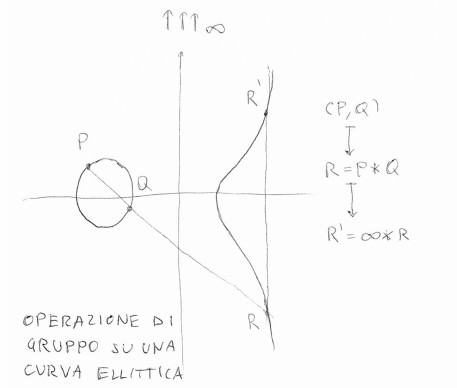
\includegraphics[width=16em]{gruppo-cubica.jpeg}

L'associatività è la proprietà più impegnativa da dimostrare. Vale la pena di notare che l'operazione è una funzione razionale delle coordinate dei punti. 
\section{Funzioni ellittiche, curve ellittiche, reticoli}
C'è una stretta correlazione tra reticoli\notamargine{Per reticoli, dove non diversmaente specificato, intendermo reticoli di rango 2 nel piano complesso}, funzioni ellittiche, curve ellittiche.

Dato un reticolo $L$, saremo in grado di costruire una funzione analitica con gruppo dei periodi L detta $\wp_L$.
D'altronde, questa speciale funzione ellittica $\wp_L$ rispetta $\wp_L'(z)^2= f_L(\wp_L(z))$ per un opportuno polinomio di terzo grado $f_L$. Perciò, la funzione $\varphi_L: z \mapsto (\wp_L'(z), \wp_L(z) )$ parametrizza una cubica $E_L$.

\begin{diagram}
 \bbC & \rTo & E_L \\
 \dTo &  \ruTo    & \\
 \bbC/L & &  \\
\end{diagram}
 
\section{Moduli}
Vogliamo cercare ora uno 'spazio dei parametri' per i tori complessi. Conosciamo già una parametrizzazione ridondante: dato un reticolo discreto $L=\omega_1 \bbZ + \omega_2 \bbZ$ possiamo costruire il toro $\bbC / L$ ( e tutti i tori sono definiti così), con $\omega_1, \omega_2$ non paralleli (ossia $\omega_1/\omega_2$ non reale). Cerchiamo ora di eliminare la ridondanza della parametrizzazione, partendo da $\mathcal{A} = \{ (\omega_1, \omega_2) \in \bbC^2: \Im(\omega_1/\omega_2) \neq 0 \} $. 

\begin{enumerate}
\item (orientazione) Anzitutto, a meno di scambiare $\omega_1, \omega_2$, possiamo supporre che $\Im(\omega_1/\omega_2) > 0$: infatti se fosse negativa, $\Im(\omega_2/\omega_1) = -\Im(\omega_1/\omega_2)  > 0$ sarebbe positiva.
\item (riscalamento) Se $\lambda \in \bbC^*$, allora $\bbC/\lambda L  \simeq \bbC/L$ tramite la mappa $z \mapsto \lambda z$ da $C/L$ in $C/\lambda L$. Dunque se $L= \omega_1\bbZ + \omega_2 \bbZ$ con $\Im(\omega_1/\omega_2) > 0$ possiamo considerare $\omega_2^{-1}L= \tau \bbZ + \bbZ $ con $\Im \tau > 0$. Ora il nostro spazio dei parametri perciò è $\mathcal{H} = \{ \tau \in \bbC: \Im \tau > 0 \} \simeq \mathcal{A} / \text{omotetie}$. Se $(\omega_1, \omega_2) \in \mathcal{A}$ indichiamo con $[\omega_1, \omega_2]$ la sua classe di equaivalenza a meno di omotetie, che ha un rappresentante privilegiato $[\omega_1/\omega_2, 1]$ in $\mathcal{H}$.
\item (cambio base) Se $M$ è una matrice 2x2 a coefficienti interi e $L=\omega_1\bbZ + \omega_2\bbZ$ è un reticolo, possiamo considerare il reticolo generato da $M[\omega_1, \omega_2]$ ($M \in End(\bbZ^2) \subset End(\bbC^2)$ agisce sulle coppie di complessi). Visto che le coppie di complessi sono a meno di omotetie, possiamo considerare $M,N \in End(\bbZ^2)$ equivalenti se esiste $\lambda \in \bbC^*$ tale che $\lambda M = N$. Il gruppo delle matrici invertibili a meno di scalari si chiama $\bbP GL_2(\bbZ)$. \notamargine{In realtà, visto che $M,N$ sono a coefficienti interi, $\lambda$ deve essere razionale.} Se $M \in \bbP GL_2(\bbZ)$, allora $M[\omega_1,\omega_2]$ è equivalente a $[\omega_1,\omega_2]$, perciò lo spazio dei parametri ora è $(\mathcal{A}/\text{omotetie})/\bbP GL_2(\bbZ)$.
\item (parametrizzazione esplicita) Così come per ogni classe di equivalenza $[\omega_1, \omega_2]$ a meno di omotetie abbiamo scelto un rappresentante privilegiato $[\tau,1]$, così scegliamo per ogni matrice $[M] \in \bbP GL_2(\bbZ)$ a meno di omotetie un rappresentante privilegiato in $SL_2(\bbQ)$. Infatti $[M*M'] = \mathrm{ Id} $ significa che esiste $\lambda \in \bbC^*$ tale che
$[M]*[M'] = \lambda \mathrm{Id} $. In particolare $\mathrm{det } M$ è invertibile, perciò possiamo scegliere $(\mathrm{det }M)^{-1}M$ equivalente a $M$ e condeterminante 1 ( e ha coefficienti in $\bbQ$). Se prendiamo ora $M \in SL_2(\bbQ)$ di coefficienti $a,b,c,d$ e lo facciamo agire su $[\tau,1]$ otteniamo $\displaystyle [a\tau+b,c\tau+d]= \left [ \frac{a\tau+b}{c \tau + d}, 1 \right ] $ .\notamargine{e si può verificare che  $\frac{a\tau+b}{c \tau + d}$ ha ancora parte immaginaria positiva.} Perciò $SL_2(\bbQ)$ agisce su $\mathcal{H}$ tramite $ M( \tau) = \frac{a \tau+b}{c\tau+d} $, e il nostro spazio dei parametri diventa infine $\mathcal{H} / SL_2(\bbQ)$.
\end{enumerate}

Dimostreremo nelle prossime lezioni che questa parametrizzazione non è più ridondante: se due tori hanno parametri diversi, allora \textit{non} sono biolomorfi. Questo seguirà dalla classificazione esplicita delle funzioni olomorfe tra tori (vedi lezione sulle isogenie).

